\section{Faster algorithm for \prob{DominatingSet}/$\sdhub[2,2]$}
\label{section:domset-22hub}

This section aims to present our current progress in finding bounds for \prob{DominatingSet}. In our effort to identify a parameter $p$ such that there exists an algorithm running in $\O^\star(3 - \varepsilon)^p$ time, we tried to extend the algorithm parameterized by $\vc$ (see \refsec{section:domset-vc}), since $\vc$ is equivalent to $\shub[1]$. While we did not succeed in developing an algorithm parameterezed by $\shub[2]$, we did find an improvement for $\prob{DominatingSet}/\sdhub[2,2]$, achieving an algorithm running in $\O^\star(2^{\sdhub[2,2]})$ time.

\medskip

Let $G$ be a graph. If $X$ is a $\sdhub[2,2]$ of $G$, then all components outside of $X$ will be called \textit{legs} due to their shapes, with $X$ considered as the \textit{body}. The number of different legs is bounded, as illustrated in \reffigure{fig:domset-22-legs}.

\begin{figure}
    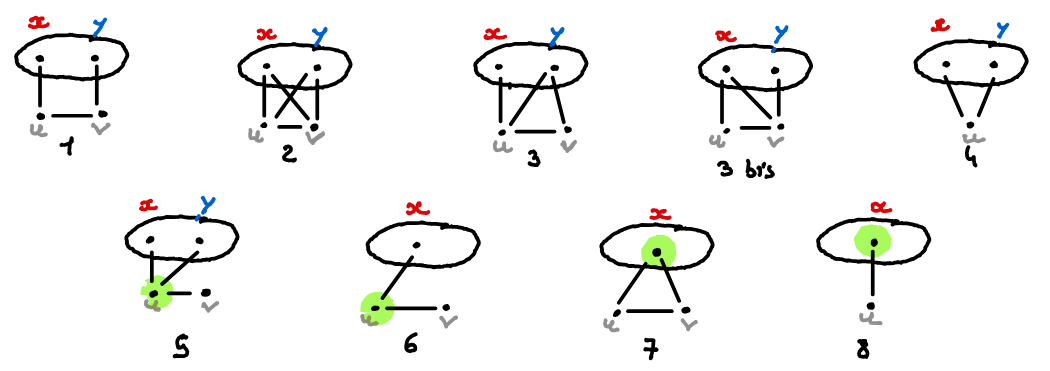
\includegraphics[width=\textwidth]{figures/domset-22-legs.png}
    \caption{All possible legs in a $\sdhub[2,2]$. Vertices of the hub $X$ are circled. The best domination for legs of types 5,6,7, and 8 is shown in green. \todo{remove the 3 bis}}
    \label{fig:domset-22-legs}
\end{figure}

We denote all the legs of $X$ by $L_1, \dots, L_m$. For the leg $L_i$, we denote the neighbours of $L_i$ in $X$ by $x_i$ and $y_i$, and the vertices of $L_i$ by $u_i$ and $v_i$, as depicted in \reffigure{fig:domset-22-legs}. We first describe the algorithm when we only have legs of type 1, then we will extend it to handle all types of legs.

\begin{lemma}
    \label{lemma:legs}
    Let $G$ be a graph and $X$ a $\sdhub[2,2]$ of $G$ where all legs are of type 1. Let $\D$ be a dominating set of minimum size for $G$ which maximizes $|\D \cap X|$. There exists no leg $L_i$ such that $|\{x_i, y_i\} \cap \D| = 1$.
\end{lemma}

\begin{proof}
    Suppose without loss of generality that $x_i \in \D$ and $y_i \notin \D$. Then, in order to dominate $v_i$, we need to take either $u_i$ or $v_i$ in $\D$. But taking $y_i$ instead of $u_i$ or $v_i$ also dominates $v_i$. Thus, since $u_i$ and $v_i$ have no other neighbours, $\D' = \D \cup \{y_i\} - \{u_i, v_i\}$ is also a dominating set of $G$ of minimum size. Morevover $|\D' \cap X| > |\D \cap X|$.
\end{proof}

Now suppose that $X \cap \D$ is known. We need to find $\D \cap (L_1, \dots, L_m)$. We will compute it using the following dynamic programming. For $A \subseteq X$ and $0 \leq i \leq m$:
$$\Phi(A, i) = \text{ a dominating set of minimum size for $A \cup L_1 \cup \dots \cup L_i$ that only uses vertices from $L_1 \cup \dots \cup L_i$}.$$

\begin{lemma}
    \label{lemma:domset-phi}
    We can compute $\Phi$ in $\O(2^{|X|}m)$ time.
\end{lemma}

\begin{proof}
    We denote $|\Phi(A, i)|$ by $\phi(A, i)$. We can compute $\phi$ with the following recurrence:
    \begin{align}
        \phi(\emptyset, 0) &= 0\\
        \phi(A, 0) &= +\infty & \text{ if } A \neq \emptyset\\
        \phi(A, i) &= \min\{1 + \phi(A \backslash \{x_i\}, i-1), 1 + \phi(A \backslash \{y_i\}, i-1), 2 + \phi(A \backslash \{x_i, y_i\}, i-1)\}
    \end{align}
    To compute $\Phi(A, i)$, follow the same dynamic programming approach: $\Phi(\emptyset, 0) = \emptyset$, $\Phi(A, 0)$ has no solution if $A \neq \emptyset$, and then track the current construction of the smallest dominating set by taking $u_i$, $v_i$ or both. We can demonstrate that $\Phi(A)$ is always one of the best dominating sets of $A \cup L_1 \cup \dots \cup L_i$:
    \begin{enumerate}
        \item $\Phi(\emptyset, 0)$ is obviously $\emptyset$.
        \item $\Phi(A, 0)$ is impossible if $A$ is not empty since we cannot take anyone in the dominating set.
        \item In order to dominate $L_i$ without using vertices of $A$, we need to take at least $u_i$ or $v_i$. If we take $u_i$, we dominates $x_i$ and can remove it from $A$; if we take $v_i$, we dominates $y_i$ and can remove it from $A$. Thus, the best solution lies between taking $u_i$, $v_i$ or both.
    \end{enumerate}
    Each computation take constant time, and there are $2^{|X|}m$ different pairs $(A, i)$. This results in an overall running time of $\O(2^{|X|}m)$.
\end{proof}

\begin{theorem}
    \label{theorem:domset-22-type1}
    Let $G$ be a graph, and let $X$ be a $\sdhub[2,2]$ of $G$ of size $|X| = l$ where all legs are of type 1. There exists an algorithm that computes $\prob{DominatingSet}/\sdhub[2,2]$ in running time $\O^\star(2^l)$.
\end{theorem}

\begin{proof}
    Consider the optimization problem of \prob{DominatingSet}: we want to find the smallest possible set of vertices that dominates $G$. The following algorithm solves this problem:

    \begin{algorithm}
        \KwData{$G = (V, E)$, $X$ a $\sdhub[2.2]$ of $G$}
        \KwResult{$\D$ a dominating set of minimum size for $G$}
        Compute $\Phi$\;
        $\D \gets V$\;
        \ForEach{$A \subseteq X$}{
            \If{for all $i$ we have $|\{x_i, y_i\} \cap A| \neq 1$}{
                $L \gets \bigcup_{|\{x_i, y_i\} \cap X| = 2}L_i$\;
                $W \gets$ vertices dominated by $A$ in $X \backslash A$\;
                $Y \gets X \backslash (A \cup W)$\;
                $D \gets (\Phi(Y, m) \backslash L) \cup A$\;
                \If{$|D|\leq |\D|$}{
                    $\D \gets D$\;
                }
            }
        }
        \caption{$\prob{DominatingSet}/\sdhub[2,2]$ that handles only legs of type 1}
        \label{algo:domset-22-1}
    \end{algorithm}

    % The number of legs $m$ does not depend on the size of $X$. However, if we have two legs $L_i$ and $L_j$ with the same neighbourhood in $X$, and we are computing $\Phi'$ for the graph $G'= G - L_j$ (which has $m-1$ legs), then when we use $\Phi(Y, m)$ (line 8), we can instead use:
    % $$\Phi(Y, m) = \Phi'(Y, m-1) \cup \{u_j\}.$$ Indeed, to dominate $L_j$, it is both necessary and sufficient to take exactly one vertex between $u_j$ and $v_j$, since all other constraints (i.e. $x_j$ and $y_j$ needing to be dominated) have already been satisfied by $L_i$. Consequently, legs with identical neighborhoods can be excluded from consideration. Thus, we only need to consider $m \leq |X|^2$ distinct legs, which is polynomial in $n$.

    % \medskip

    Since $m = \poly(n)$, the algorithm operates in time $\O^\star(2^l)$. The computation for the first line takes $\O(2^lm)$ time according to \reflemma{lemma:domset-phi}. Moreover, there are exactly $2^l$ different subsets $A \subseteq X$, and lines 4-12 can be executed in polynomial time.

    \medskip

    Now let us prove that this algorithm is correct. Consider $\D$ a dominating set of minimum size for $G$ that maximizes $|\D \cap X|$. Let $A = \D \cap X$. By \reflemma{lemma:legs}, we know there is no leg $L_i$ with one neighbour in $A$ and the other in $X \backslash A$.
    
    Let $L$ be the set of legs with two neighbours in $A$, and $W$ be all the neighbours of $A$ in $X$. Clearly, $L$ and $W$ are already dominated by $A$. Thus, with $Y = X \backslash (A \cup W)$, we need to dominate the remaining vertices, i.e., $(\bigcup_{i \leq m} L_i \backslash L) \cup Y$, without taking any element of $Y$ since we know $\D \cap X = A$.
    
    By definition, $\Phi(Y, m)$ represents a dominating set of minimum size for $\bigcup_{i \leq m} L_i \cup Y$ without taking any vertex from $X$. Furthermore, by \reflemma{lemma:legs}, $Y$ and $L$ are not connected. Thus, only one element from each leg of $L$ has been chosen in $\Phi(Y, m)$ (see \reffigure{fig:domset-22-proof}). These elements are already dominated by $A$ and are thus not usefull; this is why we need to remove them (line 8). It means that $\Phi(Y, m) \backslash L$ is a dominating set of minimum size for $(\bigcup_{i \leq m} L_i \backslash L) \cup Y$, without taking any element of $Y$ and $\D = (\Phi(Y, m) \backslash L) \cup A$. Since $A$ will be chosen in the loop (line 3), it ensures that a dominating set of minimum size will be chosen by the algorithm.

    Therefore, the algorithm correctly finds a dominating set of minimum size for $G$.

    \begin{figure}
    \centering
    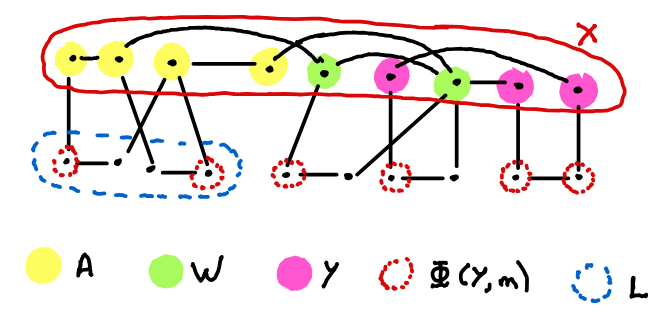
\includegraphics[width=.6\textwidth]{figures/domset-22-proof.png}
    \caption{Example of a $\sdhub[2,2]$ $X$ alongside its legs. This illustrate the best dominating set $\D = A \uplus (\Phi(Y, m) \backslash L)$ for a given $A$.}
    \label{fig:domset-22-proof}
\end{figure}
\end{proof}

Now we need to extend this algorithm to handle all types of legs.

\medskip

First, we can remove all legs of type 5, 6, 7, and 8 because we already know the optimal dominating set for these legs (see \reffigure{fig:domset-22-legs}). Note that after removing these legs, some vertices of $X$ will already be in $\D$ and others will already be dominated. From now on, we will consider there are no legs of type 5, 6, 7, and 8.

\medskip

Legs of type 2 and 4 are not problematic. Suppose $A = \D \cap X$ for a candidate $\D$. Now consider a leg $L_i$ of type 2 or 4. We have three cases: (1) both $x_i$ and $y_i$ are in $A$, then $L_i$ is fully dominated; (2) only $x_i$ or $y_i$ is in $A$, then $L_i$ is fully dominated; (3) neither $x_i$ or $y_i$ is in $A$, then taking $u_i$ always dominates $x_i$, $y_i$, and $u_i$ (and $v_i$ for type 2). Thus, we can ignore legs of types 2 and 4, as it is straightforward to determine their dominating set once $A$ is chosen.

\medskip

The remaining legs are of type 3. Once again, consider $\D$ a dominating set of minimum size for $G$ which maximizes $|X \cap \D|$ and let $A = X \cap \D$. Let $L_i$ be a leg of type 3, we have four cases: (1) $x_i$ and $y_i$ are both in $A$, then $L_i$ is fully dominated; (2) $x_i$ and $y_i$ are not in $A$, then taking $u_i$ is always the best choice since it dominates $u_i$, $v_i$, $x_i$, and $y_i$; (3) $x_i \in A$ and $y_i \notin A$, then \reflemma{lemma:legs} can apply and $\D$ does not maximizes $|X \cap \D|$; (4) $x_i \notin A$ and $y_i \in A$, then $u_i$ and $v_i$ are already dominated by $A$ and we can remove $L_i$ from consideration.

\medskip

In conclusion, we can focus only on legs of type 1. The solution with every type of legs can be computed easily thanks to the solution for legs of type 1.

\begin{theorem}
    \label{theorem:domset-22-alltypes}
    Let $G$ be a graph, and let $X$ be a $\sdhub[2,2]$ of $G$ size $|X| = l$. There exists an algorithm that computes $\prob{DominatingSet}/\sdhub[2,2]$ in running time $\O^\star(2^l)$.
\end{theorem}

\begin{proof}
    This directly follows from the observations discussed in the previous paragraphs. \refalgo{algo:domset-22-2}, which describes how to compute it, is provided in \refappendix{appendix:boring-proofs}, as its details are not particularly interesting to discuss here.
\end{proof}